\subsection{Активные и пассивные компоненты электрической цепи}

	Элементом электрической цепи называют идеализированное устройство, отображающее какое-либо из свойств реальной электрической цепи. В теории электрических цепей различают {\bfseries активные} и {\bfseries пассивные} элементы. Первые вносят энергию в электрическую цепь, а вторые ее потребляют.

\subsubsection{Пассивные компоненты электрической цепи}
\begin{itemize}
\item Резистивный элемент (резистор)

	Условное графическое изображение резистора приведено на рис. 1,а. Резистор – это пассивный элемент, характеризующийся резистивным сопротивлением. Последнее определяется геометрическими размерами тела и свойствами материала. Характеризуется сопротивлением $ R $, [Ом]  или обратной величиной, проводимостью $G = R^{-1}  $, [См] 

\begin{center}
	\begin{figure}[h!]
		\center{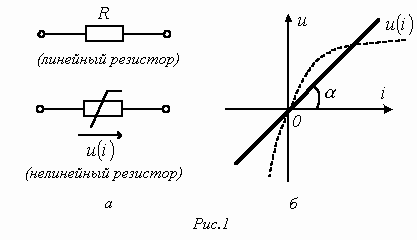
\includegraphics[scale=1]{Resistor.png}}
		\caption{ВАХ линейного и нелинейного резистора}	
	\end{figure}
\end{center}
	Основной характеристикой резистивного элемента является зависимость $u(i)$, называемая вольт-амперной характеристикой (ВАХ). Если зависимость представляет собой прямую линию, проходящую через начало координат (см.рис. 1), то резистор называется линейным и описывается соотношением
$$ R = \frac{U}{I} $$
	Нелинейный резистивный элемент, ВАХ которого нелинейна (рис. 1,б), характеризуется несколькими параметрами. В частности безынерционному резистору ставятся в соответствие статическое и дифференциальное сопротивления.
$$ R_{stat} = \frac{u}{i} $$
$$ R_{dif} = \frac{\partial u}{\partial i} $$
\item Индуктивный элемент (катушка индуктивности)

	Условное графическое изображение катушки индуктивности приведено на рис. 2,а. Катушка – это пассивный элемент, характеризующийся индуктивностью. Для расчета индуктивности катушки необходимо рассчитать созданное ею магнитное поле.

	Индуктивность определяется отношением потокосцепления к току, протекающему по виткам катушки
$$L =  \frac{\Psi}{i} $$
, [Гн]

	Связь напряжения на катушке с током, протекающим через нее:
$$ U = -L \frac{\partial i}{\partial t} $$

	Основной характеристикой катушки является Веббер-амперная характеристика:
\begin{center}
	\begin{figure}[h!]
		\center{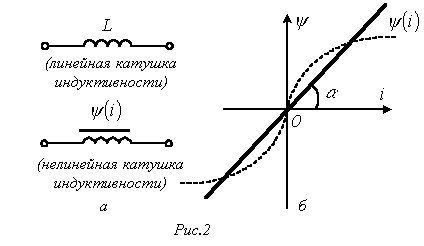
\includegraphics[scale=1]{Cat.png}}
		\caption{ Веббер-амперная характеристика катушки}	
	\end{figure}
\end{center}


	В свою очередь, катушки бывают линейными и нелинейными. Нелинейные характеризуются статической и дифференциальной индуктивностями.
 
\item  Емкостный элемент (конденсатор)
	Конденсатор – это пассивный элемент, характеризующийся емкостью. Для расчета последней необходимо рассчитать электрическое поле в конденсаторе. Емкость определяется отношением заряда q на обкладках конденсатора к напряжению u между ними
$$C = \frac{q}{u} $$
, [Ф]
	Связь напряжения на пластинах конденсатора с протекающим через него током:
$$ U = \frac{1}{C}\int i dt $$
	Условное графическое изображение конденсатора приведено на рис. 3,а.
\begin{center}
	\begin{figure}[h!]
		\center{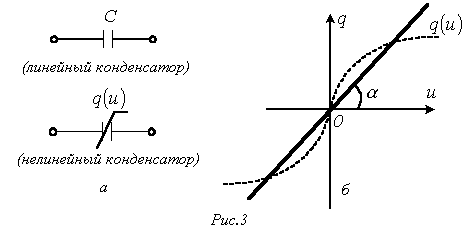
\includegraphics[scale=1]{Cond.png}}
		\caption{ Кулон-вольтная характеристика конденсатора}	
	\end{figure}
\end{center}
	Большинство диэлектриков, используемых на практике, являются линейными, а значит и конденсаторы представляют собой линейные элементы. У нелинейных диэлектриков (сегнетоэлектриков) диэлектрическая проницаемость является функцией напряженности поля, что обусловливает нелинейность зависимости $q(u)$ (рис. 3,б)
	Для нелинейных конденсаторов выделяют статическую и дифференциальную ёмкости.
\end{itemize}
\subsubsection{Активные компоненты электрической цепи}
\begin{itemize}
\item Источник напряжения (ЭДС)
\begin{center}
	\begin{figure}[h!]
		\center{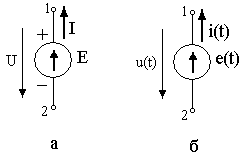
\includegraphics[scale=1]{EDS.png}}
		\caption{ Источник ЭДС}	
	\end{figure}
\end{center}

	Идеальным источником ЭДС (графическое изображение рис.4) называется активный элемент с двумя выводами (активный двухполюсник), напряжение на которых не зависит от величины тока, проходящего через источник.

	На рис.4 (а) показан источник постоянной ЭДС, а на рис.4 (б) источник переменной ЭДС.

	Выходной характеристикой элемента является вольтамперная характеристика (ВАХ). В соответствии с определение ВАХ идеального источника ЭДС это прямая линия (показана на рис. 5).
\begin{center}
	\begin{figure}[h!]
		\center{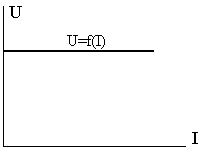
\includegraphics[scale=1.5]{EVAH.png}}
		\caption{ ВАХ Источника ЭДС}	
	\end{figure}
\end{center}
	Такая вольтамперная характеристика возможна только в том случае, если сопротивление внутренней структуры источника равно нулю.
	
	На практике идеальных источников не существует. Это объясняется наличием сопротивления во внутренней структуре источника (Rвн). Величина этого сопротивления определяется сопротивлениями соединительных проводов, коммутирующей аппаратуры, обмоток трансформаторов, внутренних структур полупроводниковых элементов и пр.

	Источник ЭДС в котором учтено внутреннее сопротивление, называется реальным источником ЭДС.

	Источник ЭДС может работать в двух режимах – в режиме генератора мощности и в режиме потребителя. В режиме генератора направление тока через источник и ЭДС совпадают, а в режиме потребителя направлены встречно.

\item Источник тока
	
	Идеальным источником тока называется активный элемент с двумя выводами (активный двухполюсник) величина тока, через который не зависит от величины приложенного к выводам напряжения. Графическое изображение источника постоянного тока показано на рис, а изображение источника переменного тока показано на рис. Вольтамперная характеристика (ВАХ) идеального источника тока показана на рис.
\begin{center}
	\begin{figure}[h!]
		\center{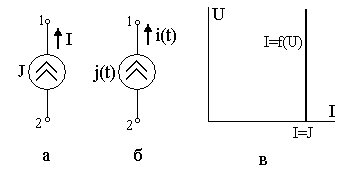
\includegraphics[scale=1.5]{I.png}}
		\caption{ Источник тока}	
	\end{figure}
\end{center}
	Такая вольтамперная характеристика возможна только в том случае, если сопротивление внутренней структуры источника равно бесконечности.

	На практике идеальных источников не существует. Это объясняется теми же причинами, что и в случае источником ЭДС.

	Источник тока в котором учтено внутреннее сопротивление, называется реальным источником тока.
\end{itemize}

\pagebreak